

\documentclass[12pt,a4paper]{article}

\usepackage[margin=2cm]{geometry}
\usepackage{amsmath,amssymb}
\usepackage{tikz}
\usetikzlibrary{shapes.geometric, positioning, arrows.meta}

\setlength{\parindent}{0pt}

\begin{document}

\begin{center}
    {\LARGE \textbf{GCSE Mathematics Recap}}
\end{center}

\vspace{1cm}

\section*{Questions}

\begin{enumerate}

    \item Alice and Bob are playing with a biased coin. The coin is biased such that $P(H) = 0.70$, what is the probability of landing on tails? As well as this, compute the probability of landing on two tails consecutively (i.e., in a row).

    \vspace{3cm}

    \item Compute the area of the following shape
   

\begin{center}
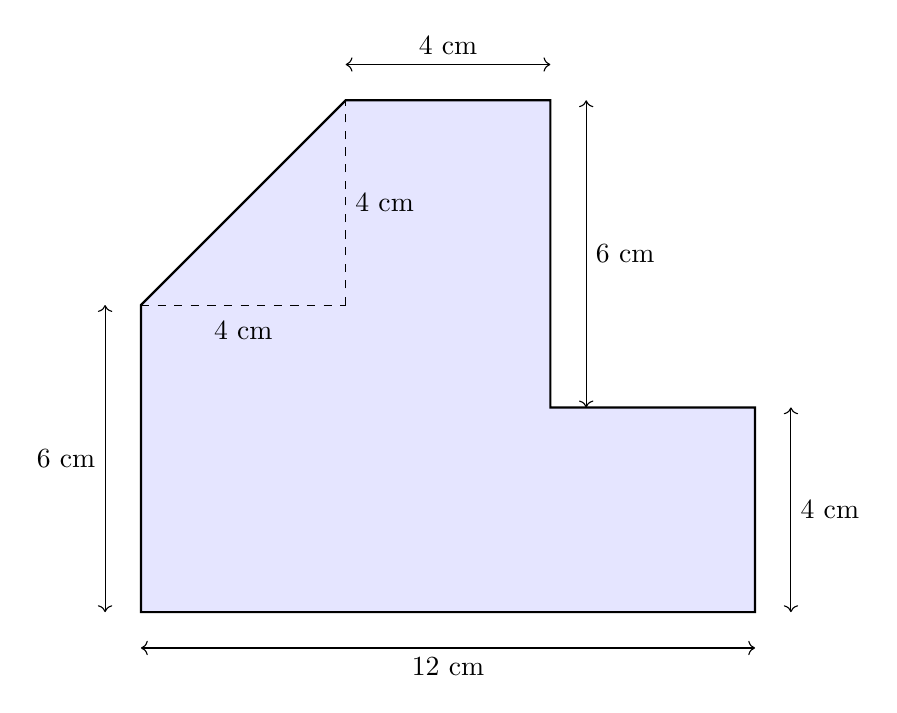
\begin{tikzpicture}[scale=0.65]

    % Shape
    \fill[blue!10]
    (0,0) -- (12,0) -- (12,4) -- (8,4)
    -- (8,10) -- (4,10) -- (0,6) -- cycle;

    \draw[thick]
    (0,0) -- (12,0) -- (12,4) -- (8,4)
    -- (8,10) -- (4,10) -- (0,6) -- cycle;

    % Bottom dimension
    \draw[<->] (0,-0.7) -- (12,-0.7);
    \node[below] at (6,-0.7) {12 cm};

    % Right vertical
    \draw[<->] (12.7,0) -- (12.7,4);
    \node[right] at (12.7,2) {4 cm};

    % Upper vertical
    \draw[<->] (8.7,4) -- (8.7,10);
    \node[right] at (8.7,7) {6 cm};

    % Top horizontal
    \draw[<->] (4,10.7) -- (8,10.7);
    \node[above] at (6,10.7) {4 cm};

    % Left vertical
    \draw[<->] (-0.7,0) -- (-0.7,6);
    \node[left] at (-0.7,3) {6 cm};

    % Diagonal horizontal and vertical components
    \draw[dashed] (0,6) -- (4,6);
    \draw[dashed] (4,6) -- (4,10);

    \node at (2,5.5) {4 cm};
    \node[right] at (4,8) {4 cm};

\end{tikzpicture}
\end{center}

\vspace{3cm}

    \item Newton's second law states that the force on an object is proportional to its acceleration,
  \begin{equation} 
   F = ma \, , 
  \end{equation}
where $m$ is the object's mass. By rearranging for $a$, show that if the mass doubles $m \to 2m$ then the acceleration must halve $a \to a/2$. Next, if the force doubles as well as the mass, show that the acceleration remains the same.
    \vspace{3cm}

    \item Alice, Bob and Dan are ordering a pizza. Alice wants to eat $30\,\text{cm}^2$ of pizza, Bob wants $15\,\text{cm}^2$, and Dan wants $40\,\text{cm}^2$.\\
    
Assuming the pizza is perfectly circular, calculate the minimum radius of the pizza they should order. Give your answer to 2 decimal places.

    \vspace{3cm}

    \item Suppose that a 4th friend joins them and wants to eat the same amount of pizza as Alice. By what percentage must the original pizza's area increase?

    \vspace{3cm}

    \item Gerald is playing darts. Given that he isn't very good, he wants to know the probability of hitting the bullseye. He models the dartboard using the following diagram. \\

The dart is equally likely to land anywhere inside the square. The dartboard is represented by the circle inscribed inside the square, and the bullseye has radius $0.25$.

\begin{center}

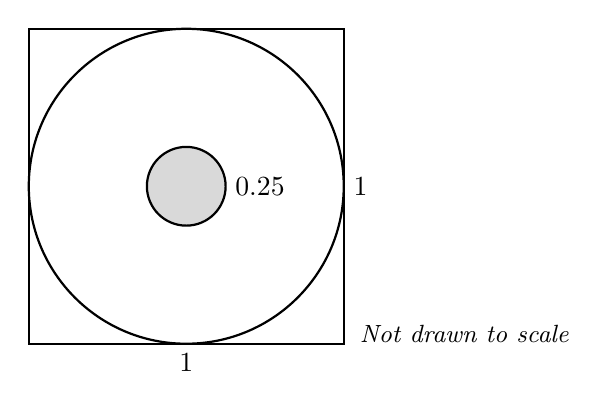
\begin{tikzpicture}[scale=4]

    % Unit square

    \draw[thick] (0,0) rectangle (1,1);

    % Dartboard

    \draw[thick] (0.5,0.5) circle (0.5);

    % Bullseye

    \fill[gray!30] (0.5,0.5) circle (0.125);

    \draw[thick] (0.5,0.5) circle (0.125);

    % Labels

    \node[below] at (0.5,0) {$1$};

    \node[right] at (1,0.5) {$1$};

    \node[right] at (0.625,0.5) {$0.25$};

    \node[right, font=\small\itshape] at (1.02,0.03) {Not drawn to scale};

\end{tikzpicture}

\end{center}

\begin{enumerate}

    \item Calculate the area of the square.

    \vspace{0.5cm}

    \item Calculate the area of the bullseye.

    \vspace{1cm}

    \item Hence, calculate the probability that Gerald hits the bullseye. Give your answer as a percentage to 2 decimal places.

    \vspace{2cm}
[\textit{hint: the probability is the ratio of the area of the bullseye to the area of the square.}]

\end{enumerate}

    \vspace{3cm}

    \item Given that 
    $4 = \sqrt{x\sqrt{x}}$. Find $x$ either by squaring or by using exponents. 

    \vspace{3cm}

    \item Given 
    \begin{equation*}
        y = \frac{8 - 3x}{4x + 9} \, ,
    \end{equation*}
    make $x$ the subject.
    
    \vspace{3cm}

    \item Solve the quadratic equation $8x^2 - 2x - 6 = 0$, given that $x > 0$.
    
    \vspace{3cm}

    \item What is the output of the following number machine?
\begin{center}
    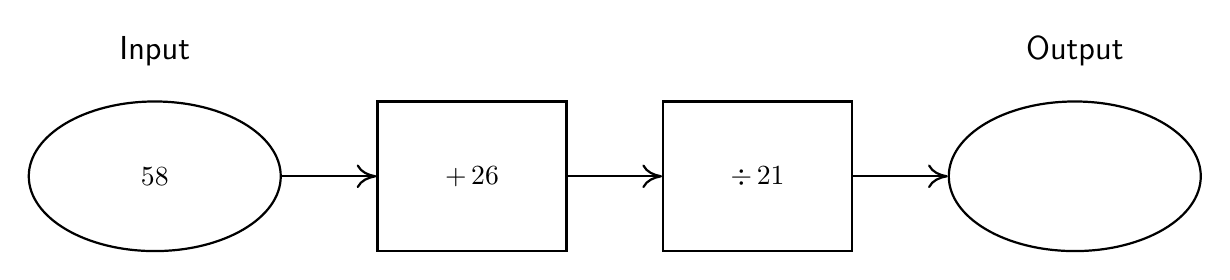
\begin{tikzpicture}[ node distance=1.2cm, thick, >={To[length=2.5mm, width=3mm]}]
  \node[ellipse, draw, minimum width=3.2cm, minimum height=1.9cm] (in) {58};
  \node[rectangle, draw, minimum width=2.4cm, minimum height=1.9cm, right=of in] (a) {$+$\,26};
  \node[rectangle, draw, minimum width=2.4cm, minimum height=1.9cm, right=of a] (b) {$\div$\,21};
  \node[ellipse, draw, minimum width=3.2cm, minimum height=1.9cm, right=of b] (out) {};
  \node[above=3mm of in, font=\sffamily\large] {Input};
  \node[above=3mm of out, font=\sffamily\large] {Output};
  \draw[->] (in) -- (a);
  \draw[->] (a) -- (b);
  \draw[->] (b) -- (out);
  \end{tikzpicture}
\end{center}


\vspace{3cm}

    \item Let $\mathbf{A}$ be an arithmetic progression, such that the first 4 terms are
    \begin{equation*}
        13 \hspace{1cm} 16 \hspace{1cm} 19 \hspace{1cm} 22
    \end{equation*}
   and let $\mathbf{G}$ be a geometric progression such that the first 4 terms are
   \begin{equation*}
        2 \hspace{1cm} 4 \hspace{1cm} 8 \hspace{1cm} 16 \, .
    \end{equation*}
   It turns out the $n$th term of $\mathbf{A}$ = 8th term of $\mathbf{G}$. Find $n$.


\vspace{3cm}

   \item A ball contains $5000\,\mathrm{cm}^3$ of air. More air is pumped into the ball at a rate of $160\,\mathrm{cm}^3$ per second. The ball is full of air when it becomes a sphere with radius $15\,\mathrm{cm}$.

\begin{center}
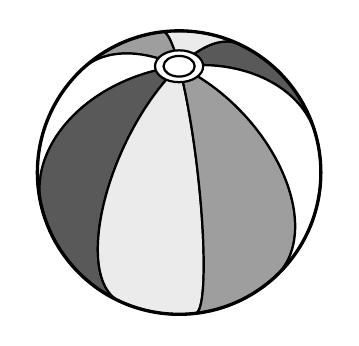
\begin{tikzpicture}[line join=round, scale=0.9]
  \def\R{2}      % radius of the drawn ball
  \def\al{48.6}  % tilt of the ball towards the viewer (degrees)
  % eight panels, each bounded by two meridians and the outline
  \foreach \k/\shade in {0/black!65, 1/black!8, 2/black!38, 3/white,
                         4/black!65, 5/black!8, 6/black!38, 7/white} {
    \pgfmathsetmacro\pa{45*\k + 10}
    \pgfmathsetmacro\pb{45*(\k+1) + 10}
    \pgfmathsetmacro\ta{atan2(cos(\al), sin(\al)*sin(\pa))}
    \pgfmathsetmacro\tb{atan2(cos(\al), sin(\al)*sin(\pb))}
    \pgfmathsetmacro\ba{atan2(sin(\ta)*sin(\pa)*cos(\al) + cos(\ta)*sin(\al), sin(\ta)*cos(\pa))}
    \pgfmathsetmacro\bb{atan2(sin(\tb)*sin(\pb)*cos(\al) + cos(\tb)*sin(\al), sin(\tb)*cos(\pb))}
    \pgfmathsetmacro\bb{ifthenelse(\bb < \ba, \bb + 360, \bb)}
    \filldraw[fill=\shade, draw=black, thick]
      plot[domain=0:\ta, samples=40, smooth, variable=\t]
        ({\R*sin(\t)*cos(\pa)}, {\R*(sin(\t)*sin(\pa)*cos(\al) + cos(\t)*sin(\al))})
      arc[start angle=\ba, end angle=\bb, radius=\R]
      -- plot[domain=\tb:0, samples=40, smooth, variable=\t]
        ({\R*sin(\t)*cos(\pb)}, {\R*(sin(\t)*sin(\pb)*cos(\al) + cos(\t)*sin(\al))})
      -- cycle;
  }
  % outline and valve
  \draw[very thick] (0,0) circle (\R);
  \filldraw[fill=white, thick] (0, {\R*sin(\al)}) ellipse ({0.34} and {0.34*cos(\al)});
  \draw[thick] (0, {\R*sin(\al)}) ellipse ({0.22} and {0.22*cos(\al)});
\end{tikzpicture}
\end{center}

How long does it take to fill the ball?

\vspace{3cm}

\item Work out
    \begin{equation*}
        2\tfrac{2}{3} \div 1\tfrac{3}{5}\,.
    \end{equation*}
    Give your answer as a mixed number in its simplest form.

    \vspace{3cm}

    \item 
    \begin{enumerate}
        \item Write $360$ as a product of its prime factors.
        \vspace{1.5cm}
        \item Hence find the highest common factor (HCF) and the lowest common multiple (LCM) of $360$ and $84$.
        \vspace{2cm}
    \end{enumerate}

    \item 
    \begin{enumerate}
        \item By rounding each number to 1 significant figure, estimate
        \begin{equation*}
            \frac{49.7 \times 0.198}{0.0512}\,.
        \end{equation*}
        \vspace{1.5cm}
        \item Work out $(3 \times 10^{5}) \times (4 \times 10^{-2})$. Give your answer in standard form.
        \vspace{1.5cm}
        \item The length of a pencil, $L$\,cm, is $7.4$\,cm correct to 1 decimal place. Write down the error interval for $L$.
        \vspace{1.5cm}
    \end{enumerate}

    \item Sam, Priya and Tom share \pounds 360 in the ratio $2 : 3 : 4$. Priya then spends $30\%$ of her share. How much money does Priya have left?

    \vspace{3cm}

    \item
    \begin{enumerate}
        \item In a sale, all prices are reduced by $20\%$. A laptop costs \pounds 552 in the sale. What was its original price?
        \vspace{2cm}
        \item Ugo invests \pounds 2500 at $3.5\%$ compound interest per year. How much interest has he earned after 4 years? Give your answer to the nearest penny.
        \vspace{2cm}
    \end{enumerate}

    \item Solve the simultaneous equations
    \begin{align*}
        3x + 2y &= 18\,,\\
        5x - 3y &= 11\,.
    \end{align*}

    \vspace{3cm}

    \item 
    \begin{enumerate}
        \item Solve $-3 < 2x + 1 \le 9$ and show your solution on the number line below.

        \begin{center}
        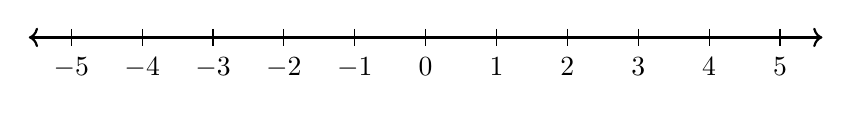
\begin{tikzpicture}[scale=0.9]
            \draw[thick, <->] (-5.6,0) -- (5.6,0);
            \foreach \n in {-5,...,5} {
                \draw (\n,0.12) -- (\n,-0.12);
                \node[below] at (\n,-0.15) {$\n$};
            }
        \end{tikzpicture}
        \end{center}

        \item List all the integers that satisfy the inequality.
        \vspace{1.5cm}
    \end{enumerate}

    \item A straight line passes through the points $(1, 5)$ and $(4, 14)$.
    \begin{enumerate}
        \item Find the equation of the line in the form $y = mx + c$.
        \vspace{2cm}
        \item Does the point $(10, 31)$ lie on the line? Explain your answer.
        \vspace{1.5cm}
    \end{enumerate}

    \item 
    \begin{enumerate}
        \item In the diagram, $AB$ is parallel to $CD$. Find the value of $x$, giving a reason for each step.

        \begin{center}
        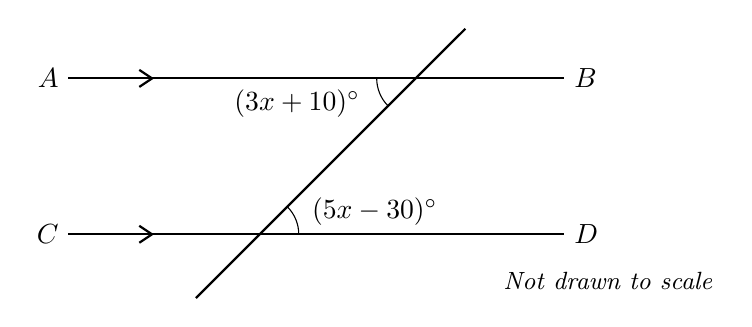
\begin{tikzpicture}[scale=0.9]
            % parallel lines with arrow marks
            \draw[thick] (0,2.2) -- (7,2.2);
            \draw[thick] (0,0) -- (7,0);
            \draw[thick] (1.0,2.32) -- (1.18,2.2) -- (1.0,2.08);
            \draw[thick] (1.0,0.12) -- (1.18,0) -- (1.0,-0.12);
            \node[left] at (0,2.2) {$A$};
            \node[right] at (7,2.2) {$B$};
            \node[left] at (0,0) {$C$};
            \node[right] at (7,0) {$D$};
            % transversal
            \draw[thick] (1.8,-0.9) -- (5.6,2.9);
            % alternate angles
            \draw (4.35,2.2) arc[start angle=180, end angle=225, radius=0.55];
            \node[left] at (4.25,1.85) {$(3x + 10)^\circ$};
            \draw (3.25,0) arc[start angle=0, end angle=45, radius=0.55];
            \node[right] at (3.3,0.32) {$(5x - 30)^\circ$};
            \node[below right] at (6.0,-0.4) {\small\textit{Not drawn to scale}};
        \end{tikzpicture}
        \end{center}

        \vspace{1.5cm}
        \item Each interior angle of a regular polygon is $156^\circ$. How many sides does the polygon have?
        \vspace{2cm}
    \end{enumerate}

    \item Triangle $ABC$ has a right angle at $B$. $AB = 7$\,cm and $BC = 24$\,cm.

    \begin{center}
    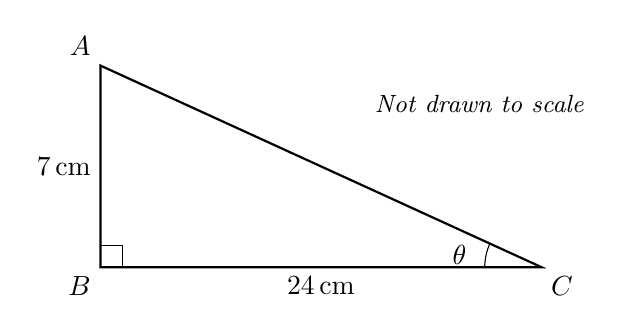
\begin{tikzpicture}[scale=0.8]
        \draw[thick] (0,0) -- (7,0) -- (0,3.2) -- cycle;
        \draw (0,0.35) -- (0.35,0.35) -- (0.35,0);
        \node[below left] at (0,0) {$B$};
        \node[below right] at (7,0) {$C$};
        \node[above left] at (0,3.2) {$A$};
        \node[left] at (0,1.6) {$7$\,cm};
        \node[below] at (3.5,0) {$24$\,cm};
        \draw (6.1,0) arc[start angle=180, end angle=155.4, radius=0.9];
        \node at (5.7,0.2) {$\theta$};
        \node[right] at (4.2,2.6) {\small\textit{Not drawn to scale}};
    \end{tikzpicture}
    \end{center}

    \begin{enumerate}
        \item Calculate the length $AC$.
        \vspace{2cm}
        \item Calculate the angle $\theta = \angle ACB$. Give your answer to 1 decimal place.
        \vspace{2cm}
    \end{enumerate}

    \item The table shows the times, $t$ minutes, that 30 students took to travel to school.

    \begin{center}
    \renewcommand{\arraystretch}{1.3}
    \begin{tabular}{|c|c|}
        \hline
        Time, $t$ (minutes) & Frequency \\
        \hline
        $0 < t \le 10$ & 4 \\
        $10 < t \le 20$ & 9 \\
        $20 < t \le 30$ & 12 \\
        $30 < t \le 40$ & 5 \\
        \hline
    \end{tabular}
    \end{center}

    \begin{enumerate}
        \item Write down the modal class.
        \vspace{1cm}
        \item Calculate an estimate of the mean time.
        \vspace{2.5cm}
        \item Explain why your answer to (b) is only an estimate.
        \vspace{1.5cm}
    \end{enumerate}

    \item The scatter graph shows the number of hours some students spent revising and their test scores.

    \begin{center}
    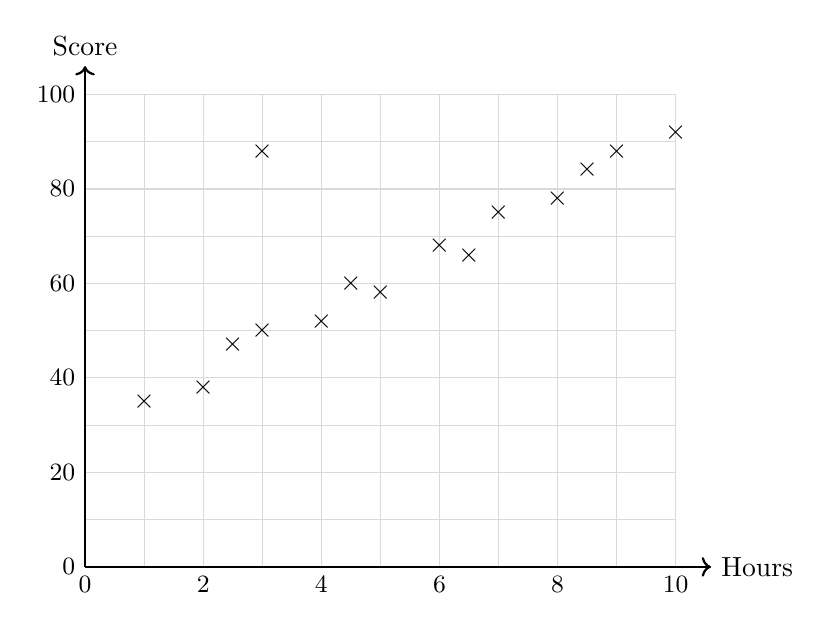
\begin{tikzpicture}[x=0.75cm, y=0.06cm]
        \draw[gray!30] (0,0) grid[xstep=1, ystep=10] (10,100);
        \draw[thick, ->] (0,0) -- (10.6,0) node[right] {Hours};
        \draw[thick, ->] (0,0) -- (0,106) node[above] {Score};
        \foreach \x in {0,2,...,10} \node[below] at (\x,0) {\small $\x$};
        \foreach \y in {0,20,...,100} \node[left] at (0,\y) {\small $\y$};
        \foreach \p in {(1,35),(2,38),(2.5,47),(3,50),(4,52),(4.5,60),(5,58),
                        (6,68),(6.5,66),(7,75),(8,78),(8.5,84),(9,88),(10,92),(3,88)}
            \node at \p {$\times$};
    \end{tikzpicture}
    \end{center}

    \begin{enumerate}
        \item Describe the type of correlation shown.
        \vspace{1cm}
        \item One student does not follow the trend. Circle this point.
        \vspace{0.5cm}
        \item Draw a line of best fit and use it to estimate the score of a student who revised for $5.5$ hours.
        \vspace{1.5cm}
        \item Explain why it would not be sensible to use your line to estimate the score of a student who revised for 20 hours.
        \vspace{1.5cm}
    \end{enumerate}

    \item A bag contains 5 red counters and 3 blue counters. Two counters are taken from the bag at random, \textbf{without} replacement.

    \begin{center}
    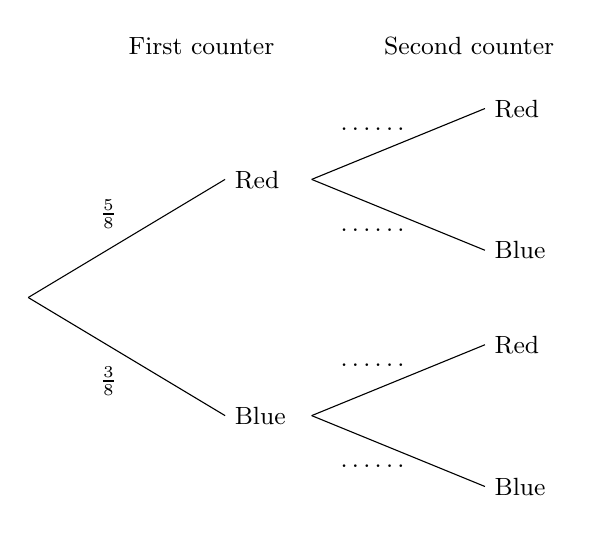
\begin{tikzpicture}[scale=1, font=\small]
        \node at (2.2,3.2) {First counter};
        \node at (5.6,3.2) {Second counter};
        \draw (0,0) -- (2.5,1.5) node[right] {Red};
        \draw (0,0) -- (2.5,-1.5) node[right] {Blue};
        \node[above left] at (1.25,0.75) {$\frac{5}{8}$};
        \node[below left] at (1.25,-0.75) {$\frac{3}{8}$};
        \draw (3.6,1.5) -- (5.8,2.4) node[right] {Red};
        \draw (3.6,1.5) -- (5.8,0.6) node[right] {Blue};
        \draw (3.6,-1.5) -- (5.8,-0.6) node[right] {Red};
        \draw (3.6,-1.5) -- (5.8,-2.4) node[right] {Blue};
        \node[above] at (4.4,2.0) {\dots\dots};
        \node[below] at (4.4,1.0) {\dots\dots};
        \node[above] at (4.4,-1.0) {\dots\dots};
        \node[below] at (4.4,-2.0) {\dots\dots};
    \end{tikzpicture}
    \end{center}

    \begin{enumerate}
        \item Complete the tree diagram.
        \vspace{0.5cm}
        \item Work out the probability that both counters are the same colour.
        \vspace{2cm}
        \item Work out the probability that at least one counter is blue.
        \vspace{2cm}
    \end{enumerate}

\end{enumerate}

\end{document}
